% mnras_template.tex 
%
% LaTeX template for creating an MNRAS paper
%
% v3.0 released 14 May 2015
% (version numbers match those of mnras.cls)
%
% Copyright (C) Royal Astronomical Society 2015
% Authors:
% Keith T. Smith (Royal Astronomical Society)

% Change log
%
% v3.0 May 2015
%    Renamed to match the new package name
%    Version number matches mnras.cls
%    A few minor tweaks to wording
% v1.0 September 2013
%    Beta testing only - never publicly released
%    First version: a simple (ish) template for creating an MNRAS paper

%%%%%%%%%%%%%%%%%%%%%%%%%%%%%%%%%%%%%%%%%%%%%%%%%%
% Basic setup. Most papers should leave these options alone.
\documentclass[fleqn,usenatbib,letters]{mnras}

% MNRAS is set in Times font. If you don't have this installed (most LaTeX
% installations will be fine) or prefer the old Computer Modern fonts, comment
% out the following line
\usepackage{newtxtext,newtxmath}
% Depending on your LaTeX fonts installation, you might get better results with one of these:
%\usepackage{mathptmx}
%\usepackage{txfonts}

% Use vector fonts, so it zooms properly in on-screen viewing software
% Don't change these lines unless you know what you are doing
\usepackage[T1]{fontenc}
\usepackage{ae,aecompl}


%%%%% AUTHORS - PLACE YOUR OWN PACKAGES HERE %%%%%

% Only include extra packages if you really need them. Common packages are:
\usepackage{graphicx}	% Including figure files
\usepackage{amsmath}	% Advanced maths commands
\usepackage{amssymb}	% Extra maths symbols

%%%%%%%%%%%%%%%%%%%%%%%%%%%%%%%%%%%%%%%%%%%%%%%%%%

%%%%% AUTHORS - PLACE YOUR OWN COMMANDS HERE %%%%%

% Please keep new commands to a minimum, and use \newcommand not \def to avoid
% overwriting existing commands. Example:
%\newcommand{\pcm}{\,cm$^{-2}$}	% per cm-squared

%%%%%%%%%%%%%%%%%%%%%%%%%%%%%%%%%%%%%%%%%%%%%%%%%%

%%%%%%%%%%%%%%%%%%% TITLE PAGE %%%%%%%%%%%%%%%%%%%

% Title of the paper, and the short title which is used in the headers.
% Keep the title short and informative.
\title[An orbit for FSR1758]{An orbit for FSR1758}

% The list of authors, and the short list which is used in the headers.
% If you need two or more lines of authors, add an extra line using \newauthor
\author[Simpson et al.]{
Jeffrey D. Simpson$^{1}$\thanks{E-mail: jeffrey.simpson@unsw.edu.au}
\\
% List of institutions
$^{1}$School of Physics, UNSW, Sydney, NSW 2052, Australia
}

% These dates will be filled out by the publisher
\date{Accepted XXX. Received YYY; in original form ZZZ}

% Enter the current year, for the copyright statements etc.
\pubyear{2019}

% Don't change these lines
\begin{document}
\label{firstpage}
\pagerange{\pageref{firstpage}--\pageref{lastpage}}
\maketitle

% Abstract of the paper
\begin{abstract}
We present an orbital calculation for the newly characterized stellar object FSR1758. This shows an object for a large motion out of the bulge and the plane of the Galaxy, with a radial distance varying from 4--16~kpc.
\end{abstract}

% Select between one and six entries from the list of approved keywords.
% Don't make up new ones.
\begin{keywords}
keyword1 -- keyword2 -- keyword3
\end{keywords}

%%%%%%%%%%%%%%%%%%%%%%%%%%%%%%%%%%%%%%%%%%%%%%%%%%

%%%%%%%%%%%%%%%%% BODY OF PAPER %%%%%%%%%%%%%%%%%%

\section{Introduction} \label{sec:intro}
The second data release of the Gaia mission \citep{GaiaCollaboration:2018io} has revolutionized our view of the Milky Way Galaxy. One of its important results is helping to confirm or refute \citep{Kos:2018we} the existence of purported stellar groupings. The precise proper motions are especially helpful in the Milky Way bugle, where photometric surveys are hampered by the large and differential reddening and extinction.

Recently \citet{Barba2018} presented a physical characterization of the large, massive stellar grouping FSR1758. Using a combination of astrometry and photometry from Gaia, DECaPS, and VVVX, they found the stellar cluster to be curiously large and could potentially be the stripped core of a dwarf galaxy. As noted by the authors, one of the key pieces of information missing were spectroscopic observations of the cluster. These are crucial for deriving a full orbit and for confirming the photometric metallicity.

In this letter we present an analysis of the orbit of FSR1758 based upon four member stars that have radial velocities (RVs) from the Gaia Radial Velocity Spectrometer (RVS).

\section{Data}

%% The "ht!" tells LaTeX to put the figure "here" first, at the "top" next
%% and to override the normal way of calculating a float position
\begin{figure*}
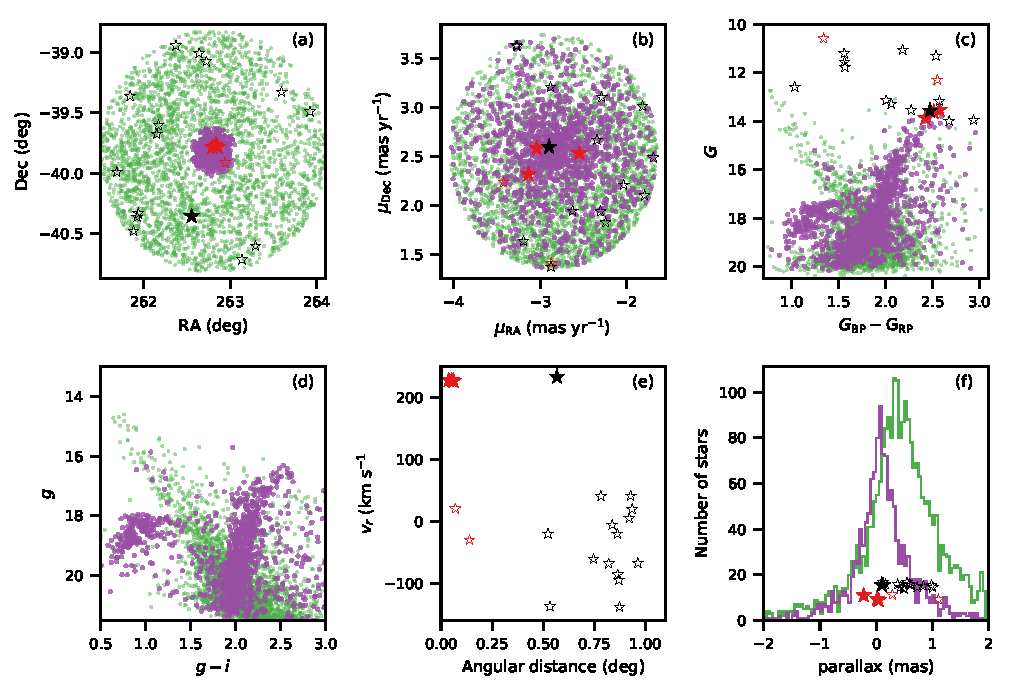
\includegraphics[width=\textwidth]{figures/cmd.pdf}
\caption{Colour-magnitude diagram of FSR1758. Blue points indicate those stars that pass the positional and proper motion criteria. The black dots are all stars within 1.5 degrees that pass just the proper motion criterium. Shown with red stars are the four members with radial velocities. \label{fig:cmd}}
\end{figure*}

An initial search was conducted for all Gaia DR2 targets within 1.0 degrees of $\mathrm{RA}=262.806^\circ, \mathrm{Dec}=-39.822^\circ$, which returned a catalogue of over 1.5 million stars. The cluster has a distinct proper motion \citep{Cantat-Gaudin2018, Barba2018}, and a sample of likely cluster members can be identified using a positional and proper motion cuts. We select our `cluster' sample as those stars within 0.20 degrees of the cluster centre, and with proper motions within 1.2 mas/yr of proper motion found by \citet{Barba2018}: $(\mu_\mathrm{RA},\mu_\mathrm{Dec})=(-2.85,2.55)$~mas/yr.

Within this sample of 1345 stars, there were five with radial velocities, with three having $226.5<v_r<227.8$~km/s. The other two stars had RV like that which would be expected along the line-of-sight --- i.e., $-100<v_r<75$~km/s. The three stars with high RV were all found at the tip of the RGB of FSR1758. This convergence of spatial, kinematic, and photometric information leads to the conclusion that three stars are members of FSR1758, and that the radial velocity of the cluster is $v_r=227\pm1$~km/s.

\citet{Barba2018} estimated the tidal radius to be $0.78\pm0.22$~deg, so we extended the search for possible members further out. Within the surrounding 1~deg, there is one further star with a large RV ($v_r=233.0$~km/s), and it is consistent with the tip of the GB. The slight discrepancy between 233~km/s and 227~km/s is consistent with the dispersion seen in other globular clusters \cite[e.g., $\omega$~Cen has a velocity dispersion of $\sim10$~km/s;][]{Johnson:2010fs}.

Unfortunately the spectra used by Gaia to measure the radial velocities was not made public in this data release. It is not possible to estimate a metallicity for the cluster from these data.

%Unfortunately the RUWE of one of these cluster members is 1.7. \citep{Lindegren2018}.

\section{Orbit}

With a radial velocity, it is now possible to estimate an orbit for FSR1758. We use the \textsc{gala} (version 0.3) \citep{M.Price-Whelan2017,Price-Whelan2018b}, with the default potential \texttt{MilkyWayPotential}. This is a simple mass-model for the Milky Way consisting of a spherical nucleus and bulge, a Miyamoto-Nagai disk, and a spherical NFW dark matter halo. The parameters of this model are set to match the circular velocity profile and disk properties of \citet{Bovy:2015gg}. We place the Sun at a Galactocentric distance of 8.2~kpc, and height above the plane of 25~pc \citep{BlandHawthorn:2016iq, Bland-hawthorn2018}. The Sun's velocity were $(U_\odot,V_\odot,W_\odot)=(11,248,7.25)$~km/s \citep{Schonrich2012}. The cluster position and velocity were $(\alpha,\delta,D_\odot,\mu_\mathrm{RA},\mu_\mathrm{Dec},v_r)=(262.806^\circ,-39.822^\circ,11.5\pm1.0~\mathrm{kpc},-2.85\pm0.1~\mathrm{mas/yr},2.55\pm0.1~\mathrm{mas/yr},227\pm1~\mathrm{km/s})$. Errors were estimated by taking 1000 samples of the error distributions and finding the 16th and 84th percentiles of the given result.

\begin{figure*}
	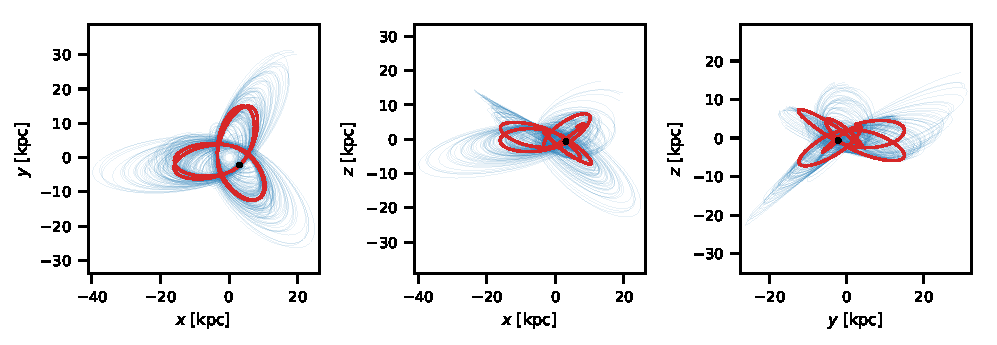
\includegraphics[width=\textwidth]{figures/orbit.pdf}
    \caption{The computed orbit for FSR1758 projected into cartesian space centred on the Galactic Centre. The red line is the orbit from the nominal values, and the blue lines show 100 orbits randomly sampling the error distributions of the input parameters. The black dot shows the position of FSR1758 as observed now.}
    \label{fig:orbit}
\end{figure*}

\begin{figure*}
	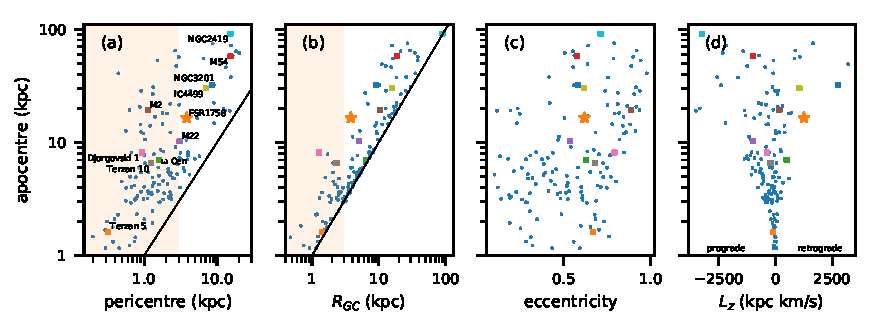
\includegraphics[width=\textwidth]{figures/orbit_comparison.pdf}
    \caption{Comparison of the orbit of FSR1758 to other globular clusters. Input parameters for all clusters were taken from \citet{Vasiliev:2018uf}, except for Djorgovski~1 and Terzan~10 which are from \citet{Ortolani2019}. In panels (a) and (b) the straight lines shows the one-to-one line. For panel (a) a cluster on this line would have a circular orbit. In panel (b) a cluster on this line is being observed at apocentre. As well as FSR1758, a number of clusters of interested are noted. Djorgovski~1 and Terzan~10 were recently found by \citet{Ortolani2019} to be halo interlopers to the bulge. The rest are multi-metallicity clusters, for which there is the potential for them to be dwarf galaxy remnants.}
    \label{fig:orbit_comparison.pdf}
\end{figure*}

The cluster is found to have a radial orbit, with a pericentre of $3.79_{-0.80}^{+0.91}$~kpc, an apocentre of $16.40_{-5.07}^{+7.48}$~kpc, and eccentricity of $0.62_{-0.04}^{+0.05}$. In Figure \ref{fig:orbit} is the plot of the previous 1~Gyr of the orbit of FSR1758 as well as 100 other possible orbits sampling the error distributions. Figure \ref{fig:orbit_comparison.pdf} shows how the orbit of FSR17578 compares to the orbit of other known clusters using data taken from \citet{Vasiliev:2018uf} for all clusters except Djorgovski~1 and Terzan~10 which is from \citet{Ortolani2019}.

FSR1758 is currently located at a Galactocentric distance of $r_g = 3.76_{-0.82}^{+1.00}$~kpc, placing at the edge of the Milky Way bulge \citep[$\sim2$~kpc across;][]{Barbuy2018}. But we find that it is not a cluster that lives in the inner Galaxy like, e.g., Terzan~5. Instead it is a halo intruder into the inner Galaxy, like Djorgovski~1 and Terzan~10 \citep{Ortolani2019}. We have caught FSR1758 at the pericentre of its orbit.

One of the unresolved questions of \citet{Barba2018} was whether FSR1758 is a dwarf galaxy or globular cluster. Overall, the orbital properties of FSR1758 do not distinguish it from other globular clusters, or potential dwarf galaxy cores (e.g., M54, $\omega$~Cen). We find that FSR1758 has quite a retrograde orbit compared to most other clusters. However it is not extreme; there are a number of clusters with $L_z > 1000$~kpc\,km/s, including objects, e.g., IC4499 has a similar angular momentum and apocentre (though much larger pericentre).

%\citet{Barba2018} found that there was a large halo of common proper motion stars around the cluster. With this in mind, we searched for evidence of a tidal streams around the cluster. To aid the search a mock stream was created using \textsc{gala} using the prescription from \citet{Fardal2015}. This enabled us to understand the evolution of proper motions and radial velocities along the stream. Being conservative, we restricted our search to within 10~deg of FSR1758. We found that stream stars within this search radius would have $v_r>180$~km/s and proper motions would remain within the 1.2 mas/yr search radius defined earlier. 

\section{Discussion}

\citet{Barba2018} claimed that there was a large halo of common proper motion stars around the cluster. However, repeating their analysis, selecting common proper motion stars along the locus of the RGB and HB, we find that many of these stars are likely field stars along the line of sight. Most are found in the colour gap between the HB and the RGB and their location in proper motion space not strongly clumped like that of the true cluster members.

Unfortunately there do not appear to have been any more serendipitous spectroscopic observations of members of this cluster. In the case of the large all-sky surveys RAVE \citep{Kunder:2017gp} and GALAH \citep{DeSilva:2015gr,Buder2018}, FSR1758 is too far into the Galactic plane for their observing footprints. Searches of the AAT, ESO, or Gemini archives fail to find any likely observations of cluster members made during bulge star surveys.

We reiterate the words of \citet{Barba2018} that ``acid test for this cluster will be to obtain spectra for a number of members''. This will enable a much better characterization of its line-of-sight velocity dispersion, metallicity, and other abundance distributions. With only four stars, it is not possible to make any comments about the radial velocity dispersion, and therefore the mass-to-light ratio of FSR1758.

\section*{Acknowledgements}

JDS acknowledges the support of the Australian Research Council through Discovery Project grant DP180101791.

%%%%%%%%%%%%%%%%%%%%%%%%%%%%%%%%%%%%%%%%%%%%%%%%%%

%%%%%%%%%%%%%%%%%%%% REFERENCES %%%%%%%%%%%%%%%%%%

% The best way to enter references is to use BibTeX:

\bibliographystyle{mnras}
\bibliography{/Users/jeffrey/Documents/library.bib}

%%%%%%%%%%%%%%%%%%%%%%%%%%%%%%%%%%%%%%%%%%%%%%%%%%

%%%%%%%%%%%%%%%%% APPENDICES %%%%%%%%%%%%%%%%%%%%%


%%%%%%%%%%%%%%%%%%%%%%%%%%%%%%%%%%%%%%%%%%%%%%%%%%


% Don't change these lines
\bsp	% typesetting comment
\label{lastpage}
\end{document}

% End of mnras_template.tex